
\documentclass{beamer}

\usepackage[T1]{fontenc}
\usepackage[utf8]{inputenc}
\usepackage[english]{babel}
\usepackage{lmodern}
% \usepackage{forloop}
\usepackage{multicol}
\usepackage{animate}
\usepackage{default}
\usepackage{listing}

\usepackage[list=true]{subcaption}
\captionsetup{compatibility=false}
\usepackage{etex}


\usepackage{tikz}
\usepackage{pgfplots}

% \usepackage{polyglossia}
% \usepackage{listings}
% \usepackage{ulem}
% \usepackage{multicol}

% \setbeamertemplate{navigation symbols}{}
% \setbeamertemplate{sidebar right}{}
% \setbeamertemplate{footline}{\hfill\insertframenumber{} | \inserttotalframenumber}


% \newcommand{\myline}{\par
%     \kern0.5pt
%     \hrule height 0.8pt
%     \kern0.5pt
% }

\usecolortheme{cormorant}
\useoutertheme{infolines}



\title[Stéganographie]{H4ck 1n TN}
\subtitle{Stéganographie : de l'âge de pierre à nos jours}
\author[H4ck1nTN]{Valentin Giannini et Vincent Noyalet}
\institute[HiT]{Ceten -- TELECOM Nancy}
\date{\today}
\logo{
\includegraphics[width=1.3cm]{logo.png}}

\begin{document}


\begin{frame}
\titlepage
% \begin{center}
% 	\includegraphics[width=3cm]{images/school-logo}
% 	\hfill
% 	\includegraphics[width=3cm]{images/logo_ul}
% 	\hfill
% 	\includegraphics[width=3cm]{images/inria}
% \end{center}
\end{frame} 

\begin{frame}{Définition (Larousse)}
	\begin{block}{Stéganographie}
		Ensemble de techniques permettant de transmettre une information en la dissimulant au sein d'une autre information (photo, vidéo, texte, etc.) sans rapport avec la première et le plus souvent anodine, essentiellement à l'aide de logiciels spécialisés.
	\end{block}

	\begin{block}{cryptographie}
	    Ensemble des techniques de chiffrement qui assurent l'inviolabilité de textes et, en informatique, de données.
	\end{block}
\end{frame}

\begin{frame}{La vieille école}
	\only<1>{
		\begin{itemize}
			\item Tablette de bois et cire
			\item Tatouage dissimulé
			\item Tissu de soie
			\item Un oeuf (oui oui)
			\item Encre invisible
			\item Mon mail
			\item Micropoint
			\item ...
		\end{itemize}
	}

	\only<2>{
		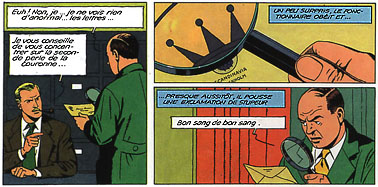
\includegraphics[scale=1.2]{meteores1.jpg}
		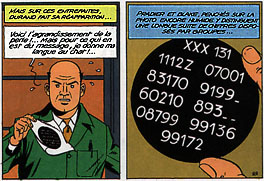
\includegraphics[scale=1.2]{meteores2.jpg}
	}

	\only<3>{
		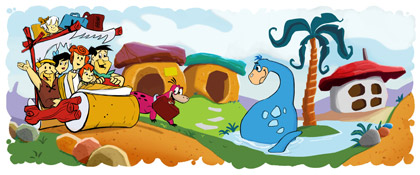
\includegraphics[scale=0.8]{pierreafeu.jpg}
	}
\end{frame}

\begin{frame}[t]{L'ère des ordinateurs}
	
	\only<1->{
		\begin{block}{Image}
			\begin{itemize}
				\item Manipulation de bits
				\item Palette de couleurs
				\item Choix d'un type de compression
			\end{itemize}
		\end{block}
	}

	\only<2->{
		\begin{block}{Texte}
			\begin{itemize}
				\item Décalage de caractères
				\item Pointer des lettres
			\end{itemize}
		\end{block}
	}

	\only<3->{
		\begin{block}{Son}
			\begin{itemize}
				\item Comme les images
				\item Jouer sur les fréquences, modulations, échantillonage, volume, steréo, ...
			\end{itemize}
		\end{block}
	}
\end{frame}

\begin{frame}{Démonstration du LSB}
	\begin{center}
		\Large Vincent c'est à toi !!!
	\end{center}	
\end{frame}


\end{document}